% respuesta2.tex

Para n=4, o 5 nodos igualmente espaciados, tenemos los siguientes polinomios que forman el spline:
\begin{align*}
S_0(x) & \text{Para x entre} -10.000000000000 \text{ y } -5.00000000 \\
S_0(x) & = 0.03846154-0.04831376(x+10.00000000)+0.00000000(x+10.00000000)^2+0.00272831(x+10.00000000)^3 \\
S_1(x) & \text{Para x entre} -5.000000000000 \text{ y } 0.00000000 \\
S_1(x) & = 0.13793103+0.15630921(x+5.00000000)+0.04092459(x+5.00000000)^2-0.00754074(x+5.00000000)^3 \\
S_2(x) & \text{Para x entre} 0.000000000000 \text{ y } 5.00000000 \\
S_2(x) & = 1.00000000+0.00000000(x-0.00000000)-0.07218643(x-0.00000000)^2+0.00754074(x-0.00000000)^3 \\
S_3(x) & \text{Para x entre} 5.000000000000 \text{ y } 10.00000000 \\
S_3(x) & = 0.13793103-0.15630921(x-5.00000000)+0.04092459(x-5.00000000)^2-0.00272831(x-5.00000000)^3
\end{align*}
Al graficar este spline, obtenemos la siguiente grafica:
\begin{figure}[H]
	\centering
	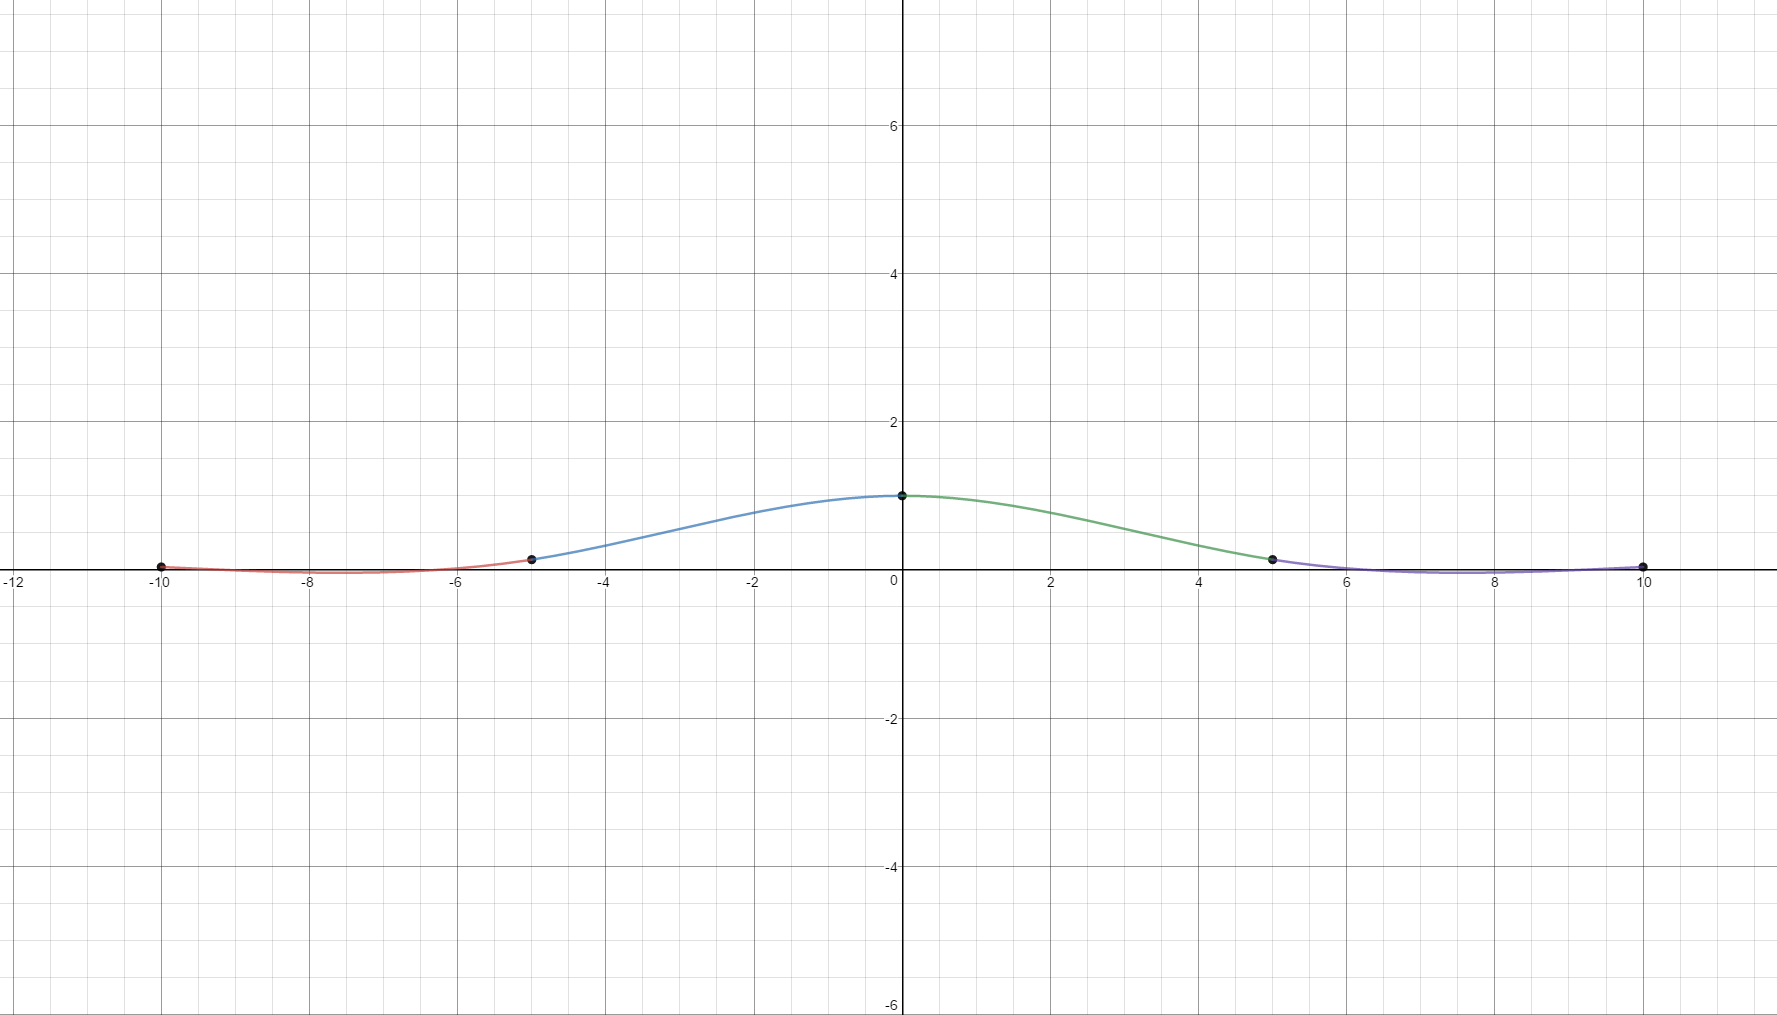
\includegraphics[scale=0.2]{img/2_4.png}
\end{figure}
Y la gráfica de este spline menos la función original:
\begin{figure}[H]
	\centering
	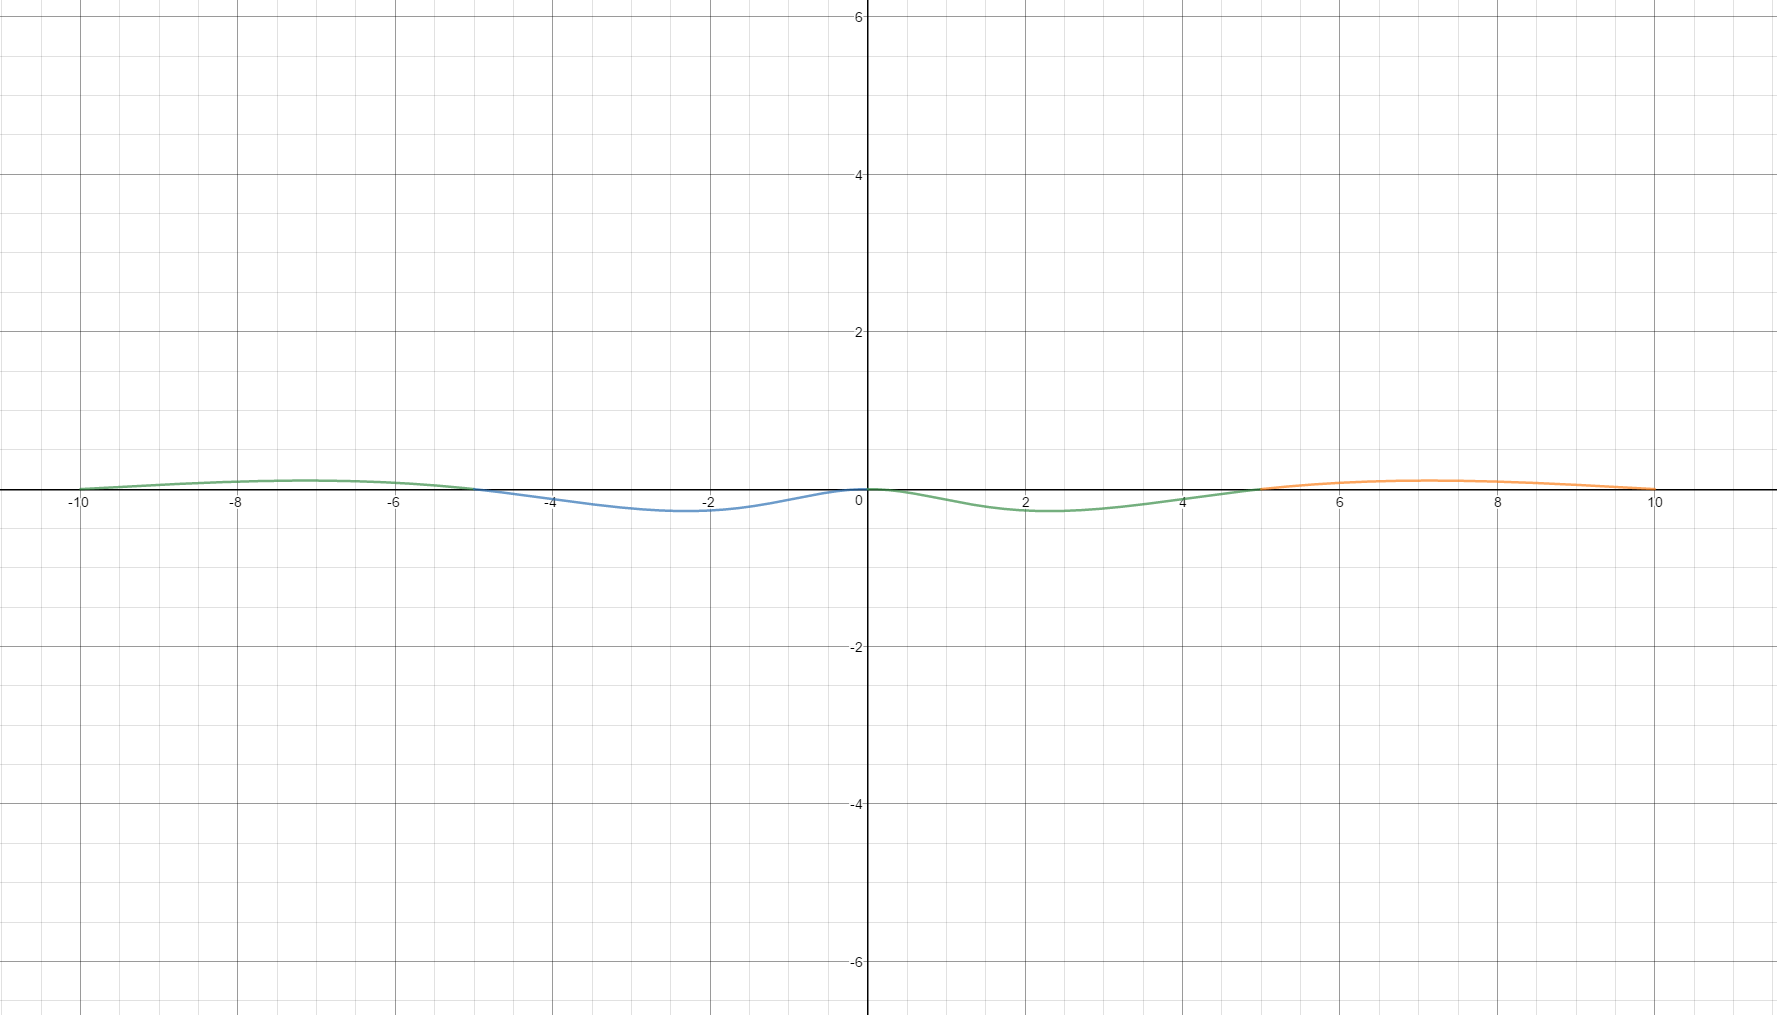
\includegraphics[scale=0.2]{img/2_4dif.png}
\end{figure}


Para n=7, o 8 nodos igualmente espaciados, tenemos los siguientes polinomios que forman el spline:
\begin{align*}
S_0(x) & \text{Para x entre} -10.000000000000 \text{ y } -7.14285714 \\
S_0(x) & = 0.03846154+0.01692967(x+10.00000000)+0.00000000(x+10.00000000)^2-0.00060590(x+10.00000000)^3 \\
S_1(x) & \text{Para x entre} -7.142857142857 \text{ y } -4.28571429 \\
S_1(x) & = 0.07270030+0.00209135(x+7.14285714)-0.00519341(x+7.14285714)^2+0.00611191(x+7.14285714)^3 \\
S_2(x) & \text{Para x entre} -4.285714285714 \text{ y } -1.42857143 \\
S_2(x) & = 0.17883212+0.12209402(x+4.28571429)+0.04719435(x+4.28571429)^2-0.01075176(x+4.28571429)^3 \\
S_3(x) & \text{Para x entre} -1.428571428571 \text{ y } 1.42857143 \\
S_3(x) & = 0.66216216+0.12846751(x+1.42857143)-0.04496363(x+1.42857143)^2+0.00000000(x+1.42857143)^3 \\
S_4(x) & \text{Para x entre} 1.428571428571 \text{ y } 4.28571429 \\
S_4(x) & = 0.66216216-0.12846751(x-1.42857143)-0.04496363(x-1.42857143)^2+0.01075176(x-1.42857143)^3 \\
S_5(x) & \text{Para x entre} 4.285714285714 \text{ y } 7.14285714 \\
S_5(x) & = 0.17883212-0.12209402(x-4.28571429)+0.04719435(x-4.28571429)^2-0.00611191(x-4.28571429)^3 \\
S_6(x) & \text{Para x entre} 7.142857142857 \text{ y } 10.00000000 \\
S_6(x) & = 0.07270030-0.00209135(x-7.14285714)-0.00519341(x-7.14285714)^2+0.00060590(x-7.14285714)^3
\end{align*}
Al graficar este spline, obtenemos la siguiente grafica:
\begin{figure}[H]
	\centering
	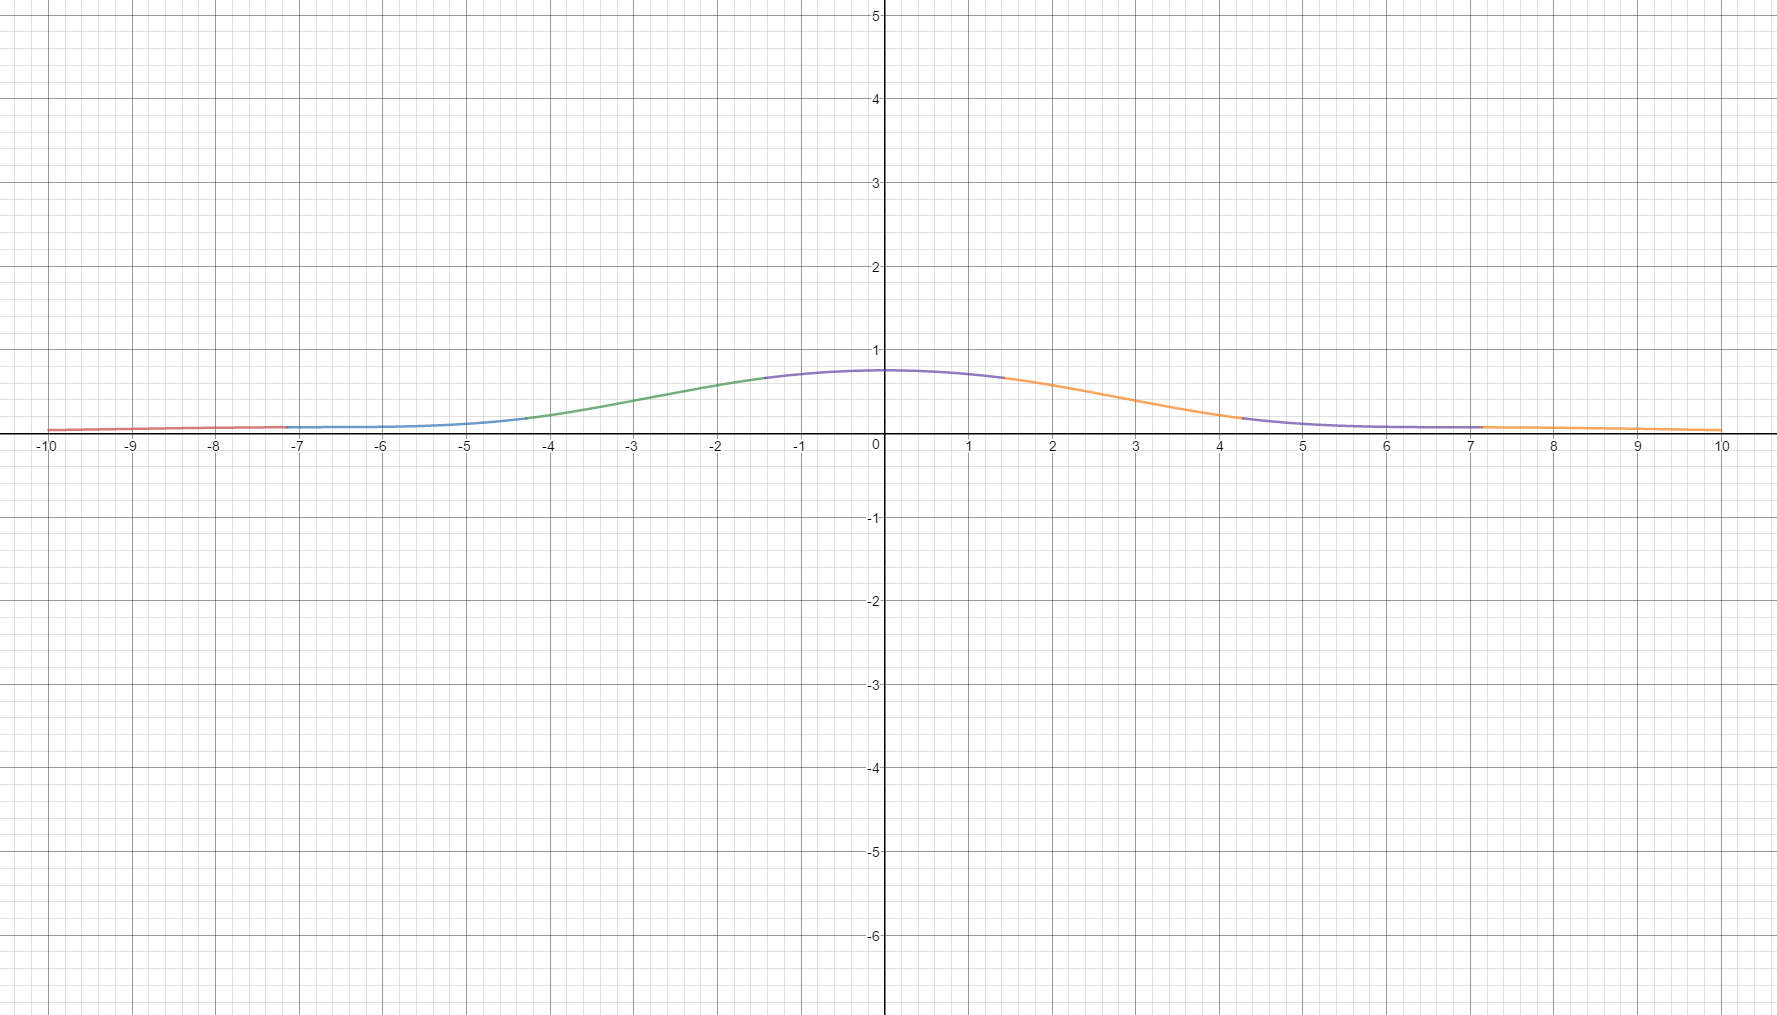
\includegraphics[scale=0.2]{img/2_7.png}
\end{figure}
Y la gráfica de este spline menos la función original:
\begin{figure}[H]
	\centering
	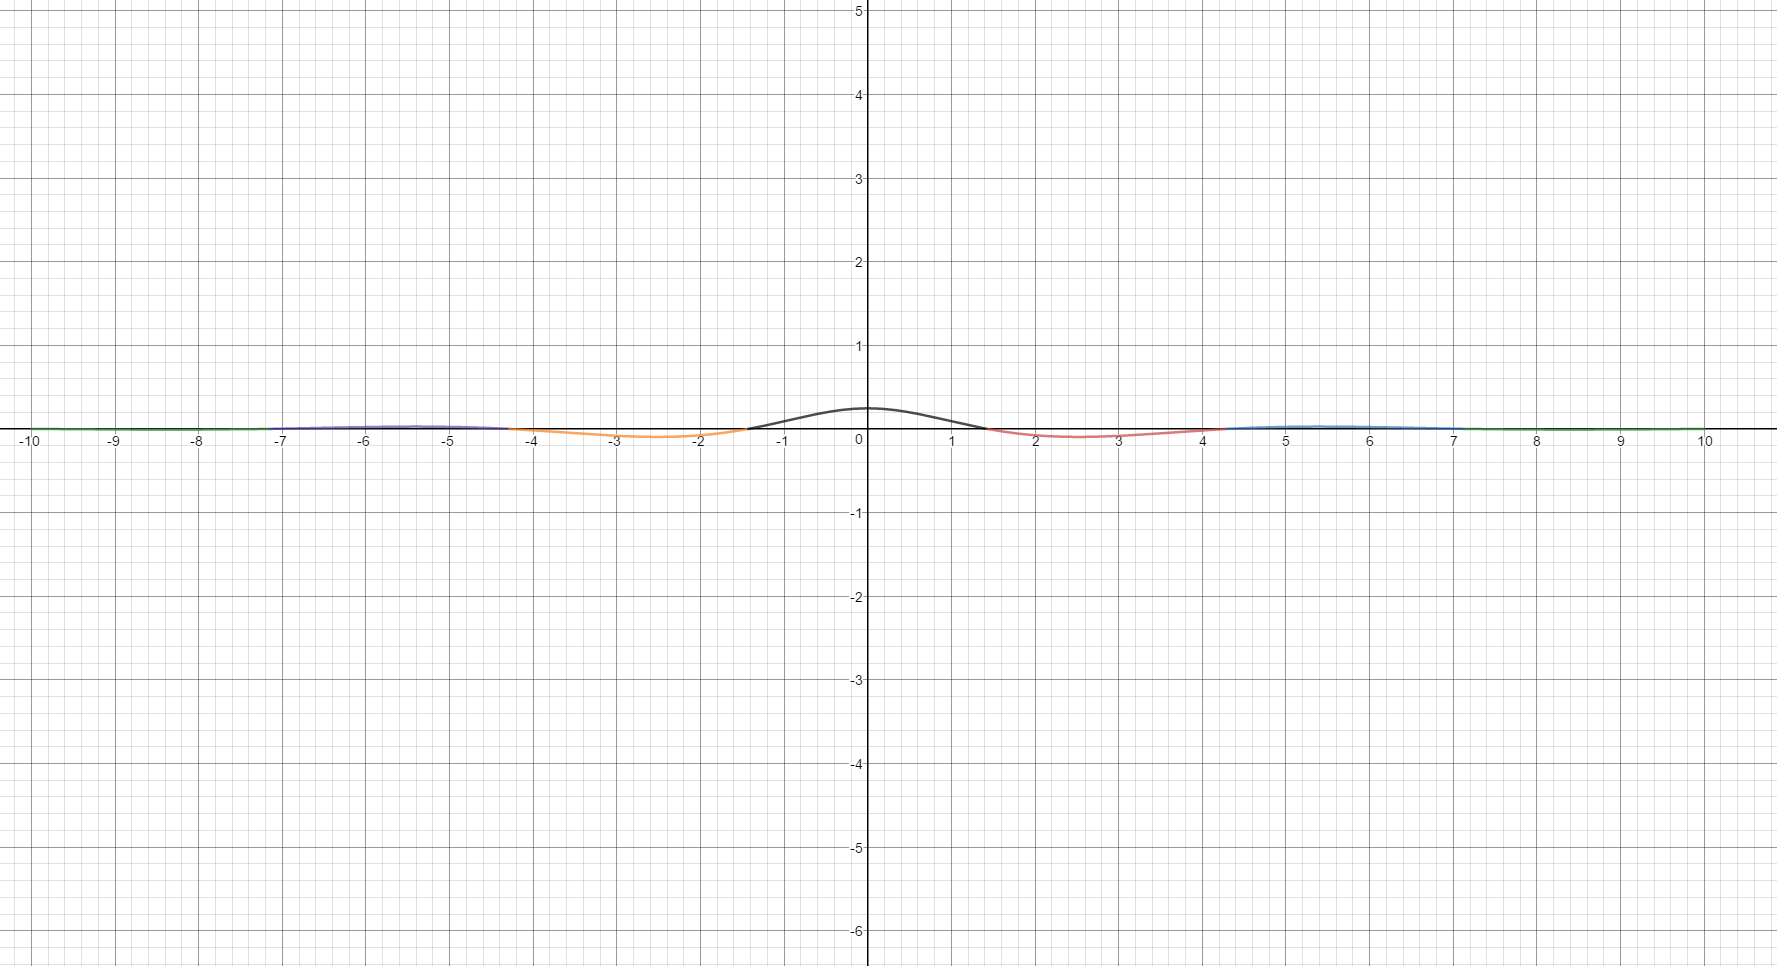
\includegraphics[scale=0.2]{img/2_7dif.png}
\end{figure}


Para n=10, o 11 nodos igualmente espaciados, tenemos los siguientes polinomios que forman el spline:
\begin{align*}
S_0(x) & \text{Para x entre} -10.000000000000 \text{ y } -8.00000000 \\
S_0(x) & = 0.03846154+0.00881415(x+10.00000000)+0.00000000(x+10.00000000)^2+0.00034171(x+10.00000000)^3 \\
S_1(x) & \text{Para x entre} -8.000000000000 \text{ y } -6.00000000 \\
S_1(x) & = 0.05882353+0.01291468(x+8.00000000)+0.00205026(x+8.00000000)^2+0.00089326(x+8.00000000)^3 \\
S_2(x) & \text{Para x entre} -6.000000000000 \text{ y } -4.00000000 \\
S_2(x) & = 0.10000000+0.03183483(x+6.00000000)+0.00740981(x+6.00000000)^2+0.00083639(x+6.00000000)^3 \\
S_3(x) & \text{Para x entre} -4.000000000000 \text{ y } -2.00000000 \\
S_3(x) & = 0.20000000+0.07151071(x+4.00000000)+0.01242813(x+4.00000000)^2+0.01340826(x+4.00000000)^3 \\
S_4(x) & \text{Para x entre} -2.000000000000 \text{ y } 0.00000000 \\
S_4(x) & = 0.50000000+0.28212232(x+2.00000000)+0.09287768(x+2.00000000)^2-0.05446942(x+2.00000000)^3 \\
S_5(x) & \text{Para x entre} 0.000000000000 \text{ y } 2.00000000 \\
S_5(x) & = 1.00000000+0.00000000(x-0.00000000)-0.23393884(x-0.00000000)^2+0.05446942(x-0.00000000)^3 \\
S_6(x) & \text{Para x entre} 2.000000000000 \text{ y } 4.00000000 \\
S_6(x) & = 0.50000000-0.28212232(x-2.00000000)+0.09287768(x-2.00000000)^2-0.01340826(x-2.00000000)^3 \\
S_7(x) & \text{Para x entre} 4.000000000000 \text{ y } 6.00000000 \\
S_7(x) & = 0.20000000-0.07151071(x-4.00000000)+0.01242813(x-4.00000000)^2-0.00083639(x-4.00000000)^3 \\
S_8(x) & \text{Para x entre} 6.000000000000 \text{ y } 8.00000000 \\
S_8(x) & = 0.10000000-0.03183483(x-6.00000000)+0.00740981(x-6.00000000)^2-0.00089326(x-6.00000000)^3 \\
S_9(x) & \text{Para x entre} 8.000000000000 \text{ y } 10.00000000 \\
S_9(x) & = 0.05882353-0.01291468(x-8.00000000)+0.00205026(x-8.00000000)^2-0.00034171(x-8.00000000)^3
\end{align*}
Al graficar este spline, obtenemos la siguiente grafica:
\begin{figure}[H]
	\centering
	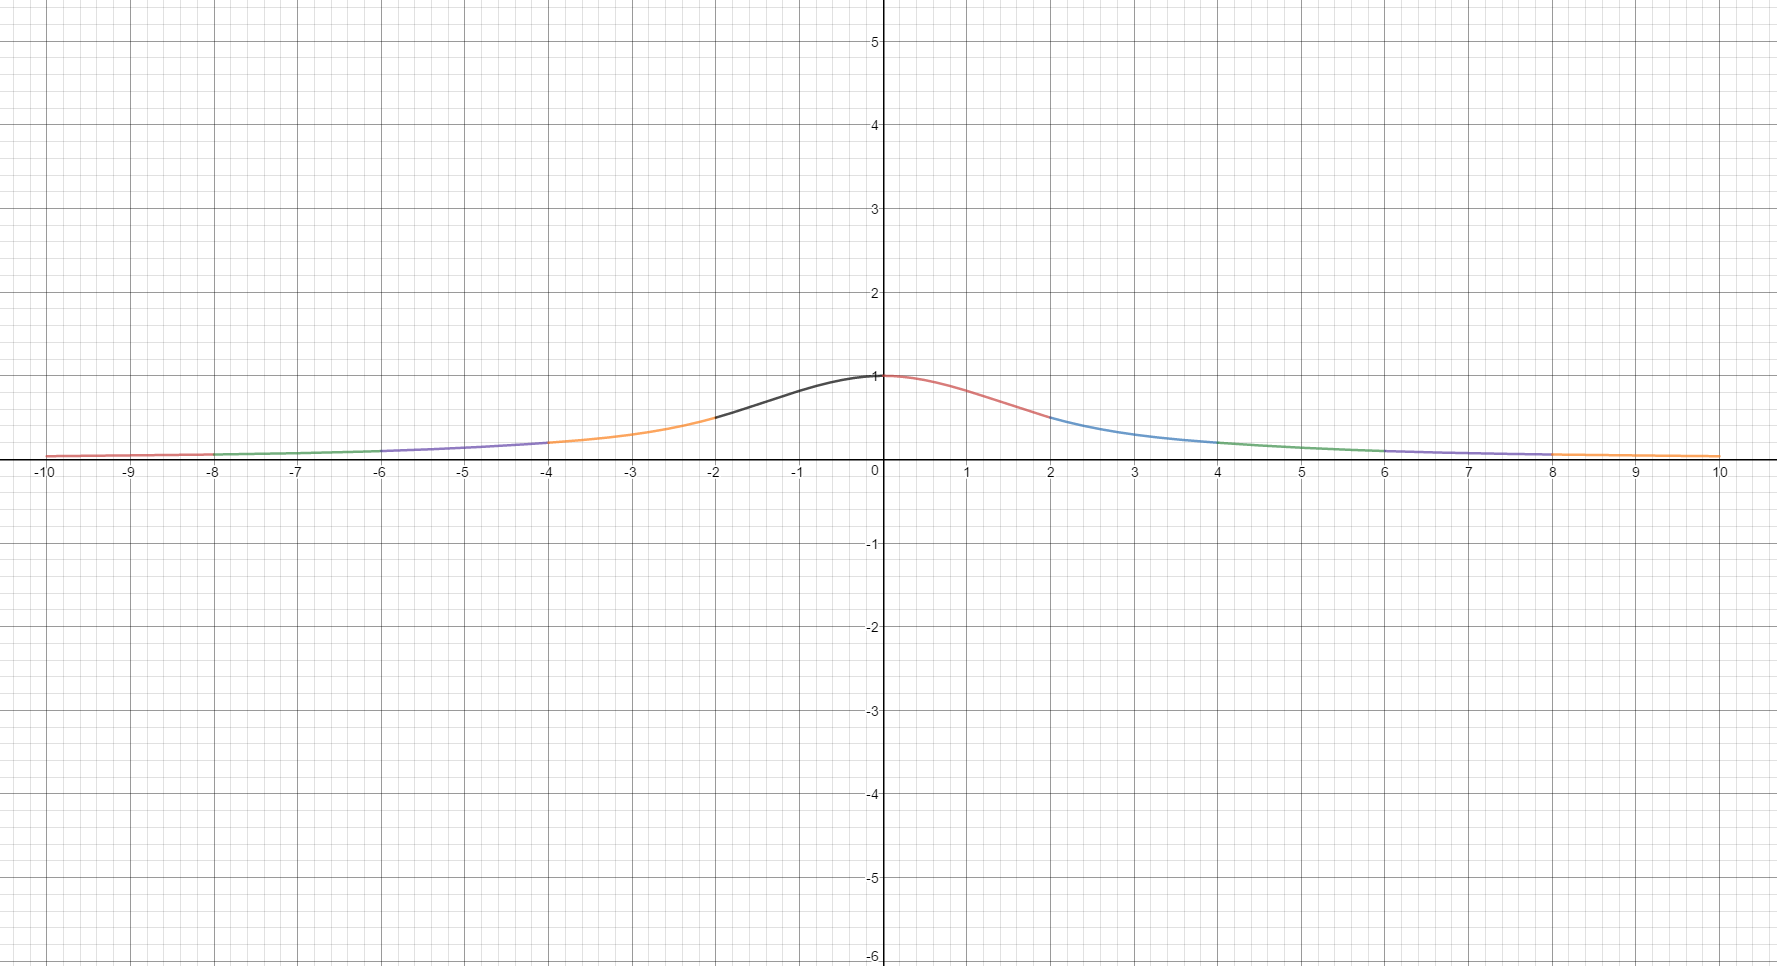
\includegraphics[scale=0.2]{img/2_10.png}
\end{figure}
Y la gráfica de este spline menos la función original:
\begin{figure}[H]
	\centering
	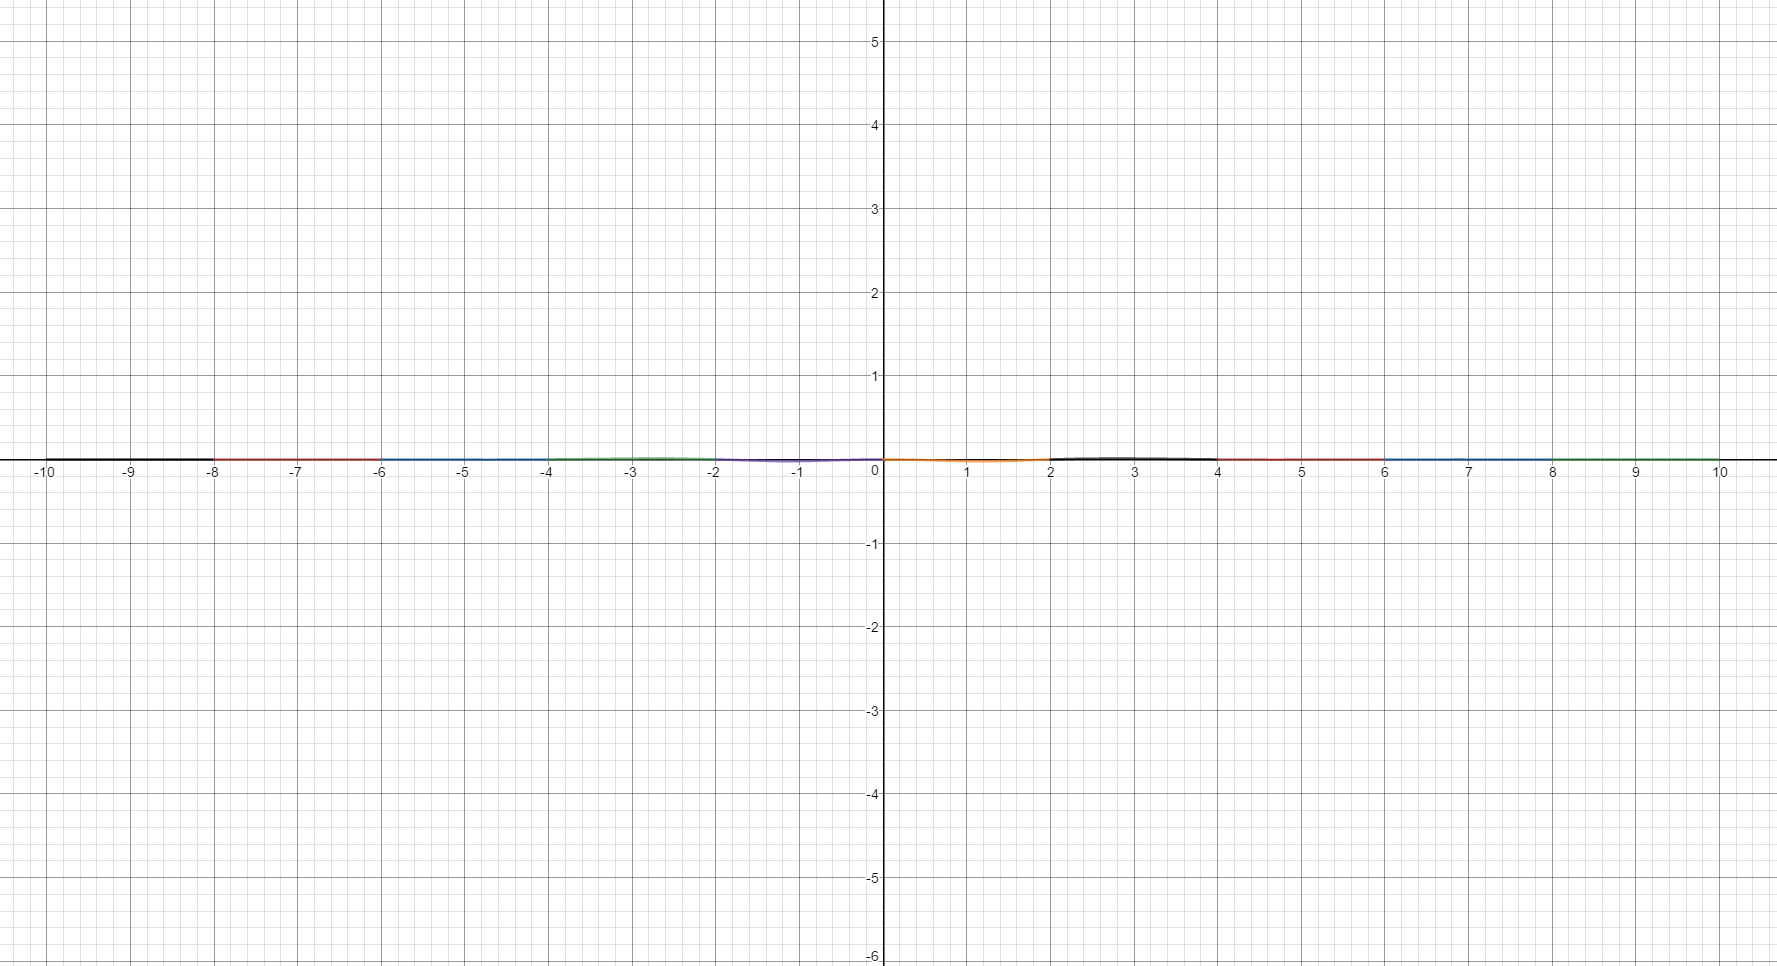
\includegraphics[scale=0.2]{img/2_10dif.png}
\end{figure}

Para observar las graficas asociadas a n=4 con mayor detalle, ingresar a \url{https://www.desmos.com/calculator/m5ivphwzin}

Para observar las graficas asociadas a n=7 con mayor detalle, ingresar a \url{https://www.desmos.com/calculator/xxtwuc6p6m}

Para observar las graficas asociadas a n=10 con mayor detalle, ingresar a \url{https://www.desmos.com/calculator/iv0a4nofql}